%%%%%%%%%%%%%%%%%%%%%%%%%%%%%%%%%%%%%%%%%
%
% (c) 2019 by Jennifer Laaser
%
% This work is licensed under the Creative Commons Attribution-NonCommercial-ShareAlike 4.0 International License. To view a copy of this license, visit http://creativecommons.org/licenses/by-nc-sa/4.0/ or send a letter to Creative Commons, PO Box 1866, Mountain View, CA 94042, USA.
%
% The current source for these materials is accessible on Github: https://github.com/jlaaser/pogil-polymers
%
%%%%%%%%%%%%%%%%%%%%%%%%%%%%%%%%%%%%%%%%%

\renewcommand{\figpath}{content/polymphys/mechanical-properties/viscoelasticity/figs}
\renewcommand{\labelbase}{viscoelasticity}

\begin{activity}{Viscoelasticity of Polymeric Materials}

\begin{instructornotes}

	This activity introduces students to the concept of viscoelasticity.
	
	After completing this activity, students will be able to:
			\begin{enumerate}
				\item Write equations connecting stress to strain and strain rate for elastic solids and viscous liquids
				\item Describe, qualitatively, what a viscoelastic liquid is
				\item Explain what is meant by ``characteristic relaxation time''
			\end{enumerate}
	
			
	\subsection*{Activity summary:}
	\begin{itemize}
		\item \textbf{Activity type:} Learning Cycle
		\item \textbf{Content goals:} Basics of viscoelasticity
		\item \textbf{Process goals:} %https://pogil.org/uploads/attachments/cj54b5yts006cklx4hh758htf-process-skills-official-pogil-list-2015-original.pdf
			\begin{itemize}
				\item Observe a physical system and reflect qualitatively on its behavior
				\item Connect qualitative observations to quantitative equations
				\item Interpret equations in terms of physical properties 
			\end{itemize}
		\item \textbf{Duration:} approx. 60 minutes
		\item \textbf{Instructor preparation required:} 
			\begin{itemize}
				\item Prepare small samples of silly putty (or comparable silicone putty) for each student group
			\end{itemize}
		\item \textbf{Related textbook chapters:}
			\begin{itemize}
				\item \emph{Polymer Chemistry} (Hiemenz \& Lodge): Sections 11.1 and 11.2.1
			\end{itemize}
	\end{itemize}

\end{instructornotes}

	%\textbf{Focus question:} Put a central question for the students to consider through this exercise here.

\begin{model}[Properties of Silicone Putty]
\label{model:sillyputty}

	Obtain a small sample of silicone putty from your instructor.
	
	Do the following experiments, and note your observations about how the material responds:
	
	\begin{enumerate}
		\item Place a small ball of putty on a table, and hit it quickly with your hand.
			\begin{itemize}
				\item Observations:
				
				\begin{solution}[1in]
				
					The putty mostly retains its shape.
					
				\end{solution}
			\end{itemize}
			
		\item Hold a small ball of putty approximately 6 inches above your desk and drop it.
			\begin{itemize}
				\item Observations:
				
				\begin{solution}[1in]
				
					The putty bounces.
					
				\end{solution}
			\end{itemize}
		
		\item Place a small ball of putty on your desk, and let it sit without touching it for 1-2 minutes.
			\begin{itemize}
				\item Observations:
				
				\begin{solution}[1in]
				
					The putty initially retains its shape, but over time, slowly begins to flow and flatten out.
					
				\end{solution}
			\end{itemize}
		
		\item Take a small piece of putty and stretch it between your hands.  Vary the rate at which you stretch it (quickly vs. slowly).
			\begin{itemize}
				\item Observations:
				
				\begin{solution}[1.25in]
				
					When the putty is pulled slowly, it stretches like taffy.
					
					When the putty is pulled quickly, it may break.
					
				\end{solution}
			\end{itemize}
		
	\end{enumerate}

\end{model}


\begin{ctqs}

	\question In which of your experiments would you say the putty behaved more like an \emph{elastic solid}?  Briefly explain your reasoning.
	
		\begin{solution}[1.25in]
		
			In experiment (1), the putty retains its shape, and is thus more solid-like.  
			
			In experiment (2), the putty bounces, which is an elastic behavior.
			
			In experiment (4), when pulled quickly, the putty ``breaks'', which is also a solid-like behavior.
		
		\end{solution}
	
	\question In which of your experiments would you say the putty behaved more like a \emph{viscous liquid}?  Briefly explain your reasoning.
	
		\begin{solution}[1in]
		
			In experiment (3), the putty flowed to match the shape of the surface it was sitting on, which is a liquid-like behavior.
		
		\end{solution}
	
	\question How did your observation of solid-like or liquid-like properties depend on the timescale on which you observed it?
	
		\begin{solution}[1in]
		
			On short timescales, the putty behaved more like a solid.
			
			On long timescales, the putty behaved more like a liquid.
			
		\end{solution}
		
	\question Explain, in one or two complete sentences, why you think we might describe this putty as a ``viscoelastic'' material.
	
			\begin{solution}[2in]
			
				We describe this putty as a viscoelastic material because it  has some properties of both elastic solids (elasticity, ability to hold its shape) and of viscous liquids (ability to flow).  The properties that we observe depend on the timescale of the observation.
				
				Note: because the liquid-like properties dominate at long times, it is appropriate to refer to the putty as a viscoelastic \emph{liquid}.
				
			\end{solution}
		
\end{ctqs}

\begin{model}[The Stress Response of Solids]

	When analyzing the response of elastic solids, we usually represent them as a spring:
	
	\vspace{3pt}
	\centerline{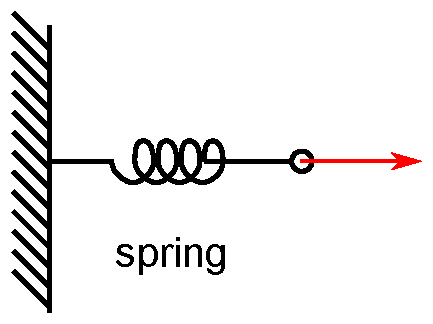
\includegraphics[width=0.3\textwidth]{\figpath/model2-spring.pdf}}
	
	An example of an elastic solid that you may be familiar with is a \emph{rubber band}.
	
\end{model}

\begin{ctqs}
	\question Suppose you take a rubber band and, at time $t=0$, you rapidly pull it to twice its original length. You then hold it at its new length. \label{\labelbase:ctq:rubberbandstepstrain}
	
		\begin{enumerate}
			\item On the following axes, sketch the force that you would expect to feel as a function of time:
			
				\begin{solution}[1.5in]
					\studentdisplay{
						\vspace{6pt}
						\centerline{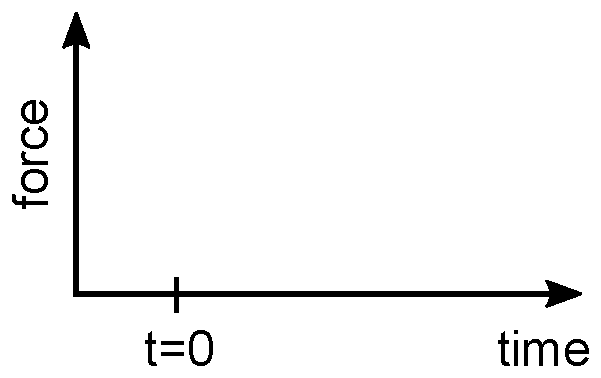
\includegraphics[width=0.4\textwidth]{\figpath/force-time-axes-blank}}
						\vspace{6pt}
					}
					\instructordisplay{
						\vspace{6pt}
						\centerline{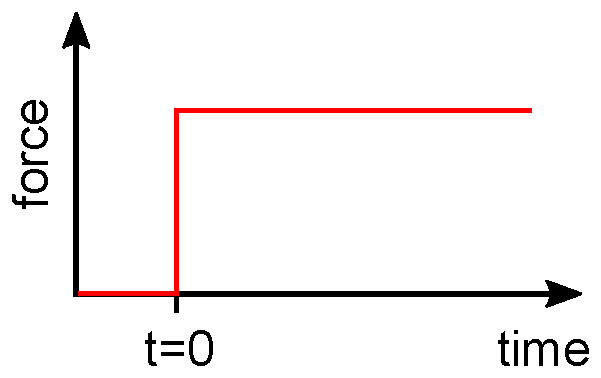
\includegraphics[width=0.4\textwidth]{\figpath/model2-spring-forcetime-solution}}
						\vspace{6pt}
					}
				\end{solution}
			
			\item Qualitatively, how is the force related to the amount of deformation?
			
				\begin{solution}[1.2in]
					The force is proportional to the amount of deformation.
				\end{solution}
			
			\item Does stretching the rubber band release energy, or require you to put energy in?
			
				\begin{solution}[1.2in]
					Stretching the rubber band requires you to put energy in (or, in other words, do work on the rubber band).
				\end{solution}
			
		\end{enumerate}
		
	\question Suppose that after holding the rubber band at double its initial length for some amount of time, you then let go of the end that you pulled.
	
		\begin{enumerate}
			
			\item What do you expect to happen to the rubber band?
			
				\begin{solution}[1in]
					The rubber band will snap back to its original length.
				\end{solution}
			
			\item Does this process release energy, or require you to put energy in?
			
				\begin{solution}[1in]
					When the rubber band snaps back, it releases energy.
				\end{solution}
			
			\item Why might we say that an elastic solid (such as the rubber band) \emph{stores} energy?  Briefly explain your answer in 1-2 complete sentences.
			
				\begin{solution}[2in]
					We say that the rubber band stores energy because, when we release it, we get back the energy that we put into the stretching process.
				\end{solution}
			
		\end{enumerate}
	
\end{ctqs}

\begin{infobox}

	Solid-like materials are typically described in terms of their \emph{modulus}, E (for extensional strain) or G (for shear strain).  For an elastic solid subjected to a strain of size $\epsilon$ (for extensional strain) or $\gamma$ (for shear strain), the resulting stress, $\sigma$, is directly proportional to the strain:
	\begin{align*}
		\sigma &= E\epsilon\,\,\,\,\,\,\,\text{(extensional strain)}\\
		%&\text{or}\\
		\text{or}\,\,\,\,\,\,\sigma &= G\gamma\,\,\,\,\,\,\,\text{(shear strain)}
	\end{align*}
	
\end{infobox}

\clearpage
\begin{ctqs}
	\question The experiment described in question \ref{\labelbase:ctq:rubberbandstepstrain} is a \emph{step strain} experiment.
	
		\begin{enumerate}
			\item A step-strain profile is shown below.  Based on the equations given above, sketch the resulting stress that you expect to measure from an elastic solid undergoing this strain:
			
				\begin{solution}[3.5in]
					\vspace{6pt}
					\centerline{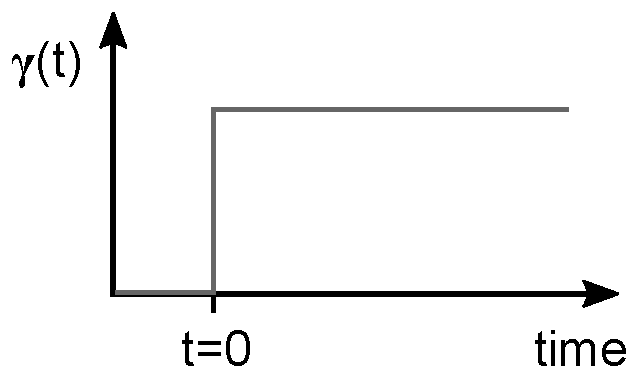
\includegraphics[width=0.45\textwidth]{\figpath/step-strain-profile}}
					\vspace{6pt}
					\studentdisplay{
						\vspace{6pt}
						\centerline{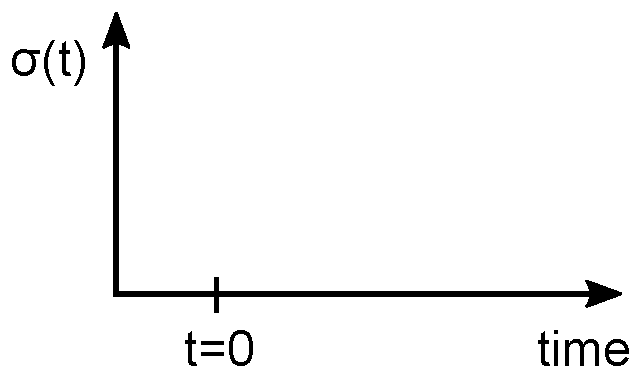
\includegraphics[width=0.45\textwidth]{\figpath/stressresponse-blank}}
						\vspace{6pt}
					}
					\instructordisplay{
						\vspace{6pt}
						\centerline{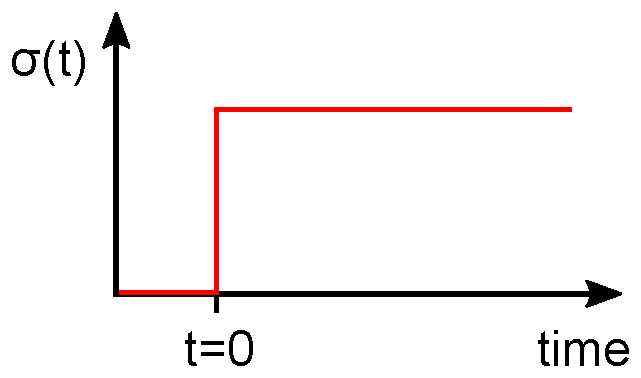
\includegraphics[width=0.45\textwidth]{\figpath/model2-spring-stressresponse-solution}}
						\vspace{6pt}
					}
				\end{solution}
				
			\item Briefly comment on whether or not your sketch from the previous question agrees with what you drew in question \ref{\labelbase:ctq:rubberbandstepstrain}.
			
				\begin{solution}[2in]
					Most students will probably get pretty close with this one, and should note that they look about the same.
				\end{solution}
		\end{enumerate}
\end{ctqs}

\clearpage
\begin{model}[The Stress Response of Liquids]

	When analyzing the response of viscous liquids, we usually represent them as a \emph{``dashpot''}:
	
	\vspace{3pt}
	\centerline{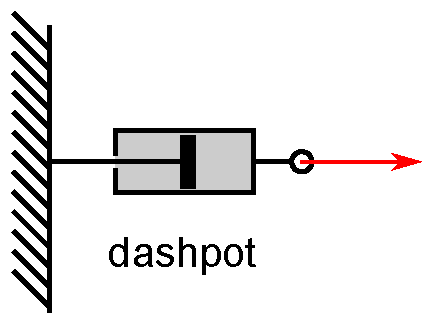
\includegraphics[width=0.3\textwidth]{\figpath/model3-dashpot.pdf}}
	
	A dashpot is just a device that contains a piece of material moving through a viscous liquid. An physical analogy for the behavior of a dashpot is moving your hand through a pool of water.
	
\end{model}

\begin{ctqs}
	
	\question  Suppose you put your hand in a pool of water. At time $t=0$, you move it rapidly one foot to the right, and then hold your hand in its new position.\label{\labelbase:ctq:poolstepstrain}
	
		\begin{enumerate}
			\item On the following axes, sketch the force that you would expect to feel as a function of time:
			
				\begin{solution}[1.5in]
					\studentdisplay{
						\vspace{6pt}
						\centerline{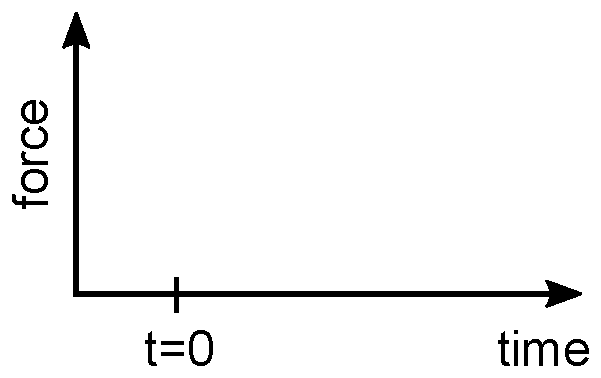
\includegraphics[width=0.4\textwidth]{\figpath/force-time-axes-blank}}
						\vspace{6pt}
					}
					\instructordisplay{
						\vspace{6pt}
						\centerline{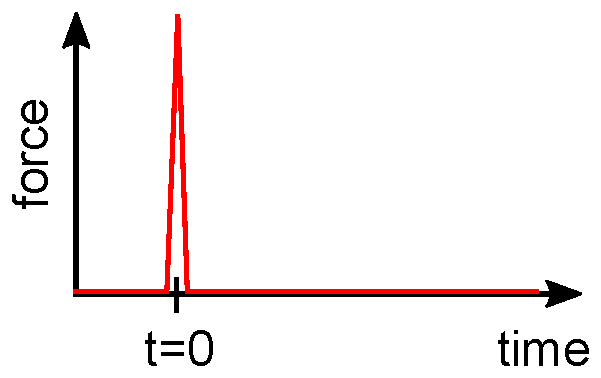
\includegraphics[width=0.4\textwidth]{\figpath/model3-dashpot-forcetime-solution}}
						\vspace{6pt}
					}
				\end{solution}
			
			\item Qualitatively, is the force more closely related to the \emph{amount} of displacement, or the \emph{rate} of displacement?
			
				\begin{solution}[1.2in]
					The force is proportional to the rate of movement.
				\end{solution}
			
			\item Does moving your hand through the water release energy, or require you to put energy in?
			
				\begin{solution}[1.2in]
					Moving your hand through the water requires you to put energy in.
				\end{solution}
				
			\item As you hold your hand in its new position, what happens to the force you feel?
			
				\begin{solution}[1in]
					The force goes to zero (or, drops down to just the hydrostatic pressure of the surrounding water).
				\end{solution}
			
		\end{enumerate}
		
	\question Suppose that after holding your hand in its new position for some amount of time, you then rapidly move it back to its original position.
	
		\begin{enumerate}
			
			\item Does this process release energy, or require you to put energy in?
			
				\begin{solution}[1in]
					When you move your hand back to its original position, you have to put more energy in.
				\end{solution}
			
			\item Why might we say that a viscous liquid (such as the water in the pool) \emph{dissipates} energy? Briefly explain your answer in 1-2 complete sentences.
			
				\begin{solution}[2in]
					We say that the viscous liquid dissipates energy because we cannot get back the energy that we originally put in - it is quickly converted to random motion of the water molecules, and cannot do further directional work.
				\end{solution}
			
		\end{enumerate}
	
\end{ctqs}

\begin{infobox}
	
	Liquid-like materials are typically described in terms of their \emph{viscosity}, $\eta$.  For a liquid, the stress is proportional to the strain \emph{rate}:
	\begin{align*}
		\sigma &= \eta\frac{d\epsilon}{dt}=\eta\dot\epsilon\,\,\,\,\,\,\,\text{(extensional strain)}\\
		%&\text{or}\\
		\text{or}\,\,\,\,\,\,\sigma &= \eta\frac{d\gamma}{dt}=\eta\dot\gamma\,\,\,\,\,\,\,\text{(shear strain)}
	\end{align*}

\end{infobox}

\clearpage
\begin{ctqs}

	\question The experiment described in question \ref{\labelbase:ctq:poolstepstrain} is again a step strain experiment.
	
		\begin{enumerate}
			\item Based on the equations given above, sketch the stress you expect to measure from a viscous liquid undergoing a step strain (the strain profile is reproduced below for reference):
			
				\begin{solution}[3.5in]
					\vspace{6pt}
					\centerline{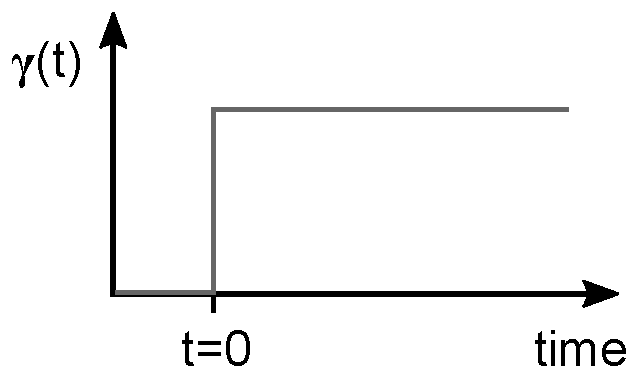
\includegraphics[width=0.45\textwidth]{\figpath/step-strain-profile}}
					\vspace{6pt}
					\studentdisplay{
						\vspace{6pt}
						\centerline{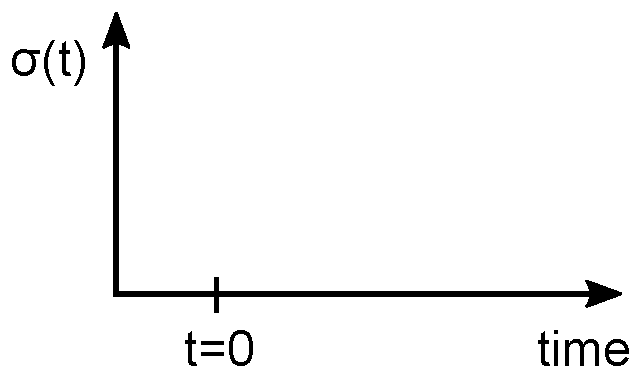
\includegraphics[width=0.45\textwidth]{\figpath/stressresponse-blank}}
						\vspace{6pt}
					}
					\instructordisplay{
						\vspace{6pt}
						\centerline{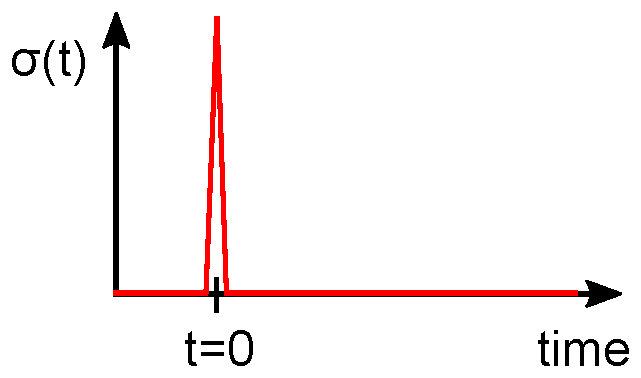
\includegraphics[width=0.45\textwidth]{\figpath/model3-dashpot-stressresponse-solution}}
						\vspace{6pt}
					}
				\end{solution}
				
			\item Briefly comment on whether or not your sketch from the previous question agrees with what you drew in question \ref{\labelbase:ctq:poolstepstrain}.
			
				\begin{solution}[1in]
					Students will likely get the qualitative features of the plot right, but may not have made the peak at $t=0$ sharp enough, or may no have drawn the force as going to $0$ as $t\to\infty$.
				\end{solution}
		\end{enumerate}
\end{ctqs}
	
\clearpage
\begin{model}[The Maxwell Model]
\label{\labelbase:mdl:maxwell}

	One simple way to describe the viscoelasticity of polymeric materials is to imagine the response of the material as being represented by a spring \emph{and} a dashpot, connected in series
	
	\vspace{3pt}
	\centerline{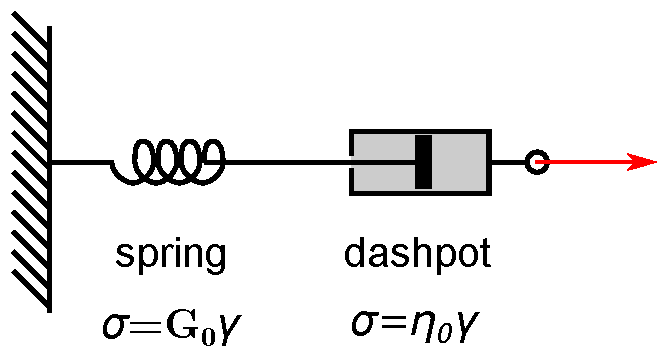
\includegraphics[width=0.5\textwidth]{\figpath/model4-maxwell}}
	
	This model is called the \emph{Maxwell element}; in this model, the spring represents the elastic solid-like portion of the material's response, while the dashpot represents the viscous liquid-like portion of the material's response.
	
\end{model}

	
\begin{ctqs}
	\question Suppose we perform a step-strain experiment on the Maxwell element, in which we rapidly pull the handle some distance to the right at $t=0$ and then hold it in its new position.
	
		\begin{enumerate}
			\item In one or two complete sentences, describe what you expect to happen in the instant immediately after you pull on the handle:
			
				\begin{solution}[1.75in]
					Initially, the spring will stretch, but the dashpot will not because it cannot respond as quickly.
				\end{solution}
			
			\item In one or two complete sentences, describe what you expect to happen as you hold the handle in its new position:
			
				\begin{solution}[1.75in]
					As the handle is held in its new position, the material in the dashpot will begin to move, and the spring will slowly contract back to its original position.
				\end{solution}
			
			\item Sketch the force that you would expect to feel as a function of time: \label{\labelbase:ctq:maxwellstepstrain}
			
				\begin{solution}[1.75in]
					\studentdisplay{
						\vspace{6pt}
						\centerline{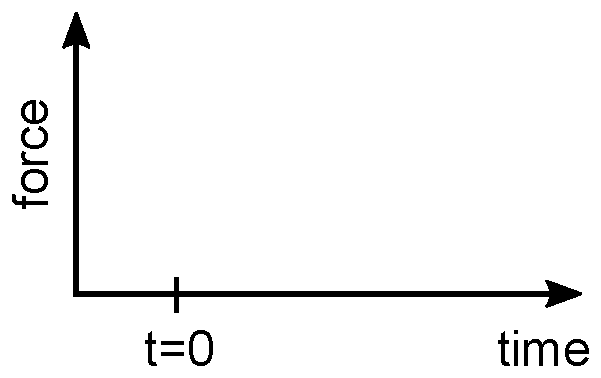
\includegraphics[width=0.45\textwidth]{\figpath/force-time-axes-blank}}
						\vspace{6pt}
					}
					\instructordisplay{
						\vspace{6pt}
						\centerline{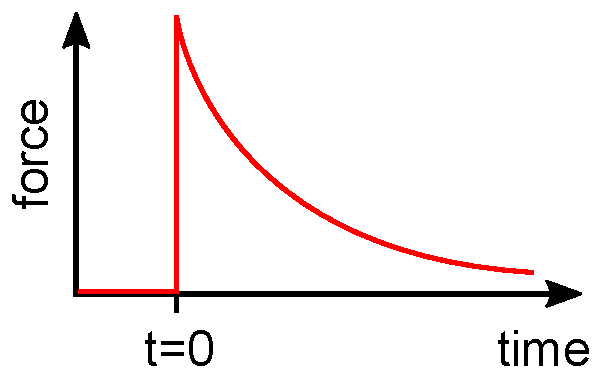
\includegraphics[width=0.45\textwidth]{\figpath/model4-maxwell-forcetime-solution}}
						\vspace{6pt}
					}
				\end{solution}
		\end{enumerate}
					
\end{ctqs}

\begin{infobox}
	As shown in Exercise \ref{\labelbase:exc:maxwell}, the time-dependent stress for a step-strain experiment on a Maxwell element works out to be:
	\begin{align*}
		\sigma(t) = \sigma_0 e^{-t G_0/\eta_0}  && \text{or} && \sigma(t) = \sigma_0 e^{-t /\tau}
	\end{align*}
	where $\tau = \eta_0/G_0$.
\end{infobox}

\begin{ctqs}
	
	\question Is this equation consistent with your prediction from question \ref{\labelbase:ctq:maxwellstepstrain}?  Why or why not?
	
					\begin{solution}[1.75in]
					
						Most students will have gotten the graph qualitatively correct, but may miss some details (such as the sharp spike in the stress at $t=0$, or the decay all the way to zero).
					
					\end{solution}
		
	\question At what time $t$ will $\sigma(t)$ drop to 1/e of its initial value?
	
					\begin{solution}[1.75in]
						The initial value of $\sigma$ is $\sigma_0$.  $\sigma(t) = \sigma_0/e$ when
						\begin{align*}
							\frac{\sigma_0}{e} &= \sigma_0 e^{-t/\tau} \\
							\frac{1}{e} &= e^{-t/\tau}\\
							e^{-1} &= e^{-t/\tau}\\
							-1 &= -\frac{t}{\tau} \\
							t &= \tau
						\end{align*}
					\end{solution}
		
		\question Why might we refer to $\tau$ as the ``characteristic relaxation timescale''?  Explain your reasoning in 1-2 complete sentences.
	
					\begin{solution}[1.5in]
					
						$\tau$ is a timescale that depends on the properties of the material, $G_0$ and $\eta_0$.  Any measurement of this material will give the same relaxation time, so we say this timescale is characteristic of the material.
					
					\end{solution}
					
		\question The silicone putty that you investigated at the beginning of this activity has a characteristic relaxation timescale of approximately 10 minutes.
		
			\begin{enumerate}
				\item On timescales \emph{shorter} than this characteristic relaxation time, did the putty appear to be more liquid-like or more solid-like?
	
					\begin{solution}[0.75in]
					
						The putty appeared to be more solid-like on short observation timescales.
						
					\end{solution}
				
				\item On timescales \emph{longer} than this characteristic relaxation time, did the putty appear to be more liquid-like or more solid-like?
	
					\begin{solution}[0.75in]
					
						The putty appeared to be more liquid-like over long observation timescales.
						
					\end{solution}
				
				\item In 2-3 complete sentences, briefly summarize the relationship between the characteristic relaxation time, the timescale of your observation, and the perceived liquid-like or solid-like properties of the material.
	
					\begin{solution}[2.5in]
					
						Generally, measurements that observe the material on timescales shorter than the characteristic relaxation time will observe solid-like properties, because the material does not have time to dissipate energy on the timescale of the measurement.
						
						By contrast, measurements that observe the material on timescales longer than the characteristic relaxation time will observe liquid-like properties, because the material can dissipate energy on the timescale of the measurement.
					
					\end{solution}
			\end{enumerate}
		
\end{ctqs}
	

%\clearpage
\begin{exercises}

		\exercise Viscoelastic properties can arise from a number of molecular-scale interactions.  Which of the following do you think would give rise to viscoelastic properties in a polymeric material?  For each interaction that you think would cause a viscoelastic response, identify the physical process that you think would be most closely associated with the relaxation time of the material.
		
			\begin{enumerate}
				\item Covalent crosslinking of the polymer chains
				
					\begin{solution}\instructordisplay{
						Covalent crosslinking will primarily lead to an \emph{elastic} response in the material.  Motion of the chain segments, dangling ends, etc. may still contribute a viscous portion to the response; because the elastic response dominates the long-time behavior, however, this material will primarily behave as a viscoelastic \emph{solid} rather than a viscoelastic \emph{liquid} (see Exercise \ref{\labelbase:exc:voigt}).
					}\end{solution}
					
				\item Hydrogen bonds (or other ``sticky'' noncovalent interactions) between polymer chains
				
					\begin{solution}\instructordisplay{
						Yes, this is likely to lead to a viscoelastic response.  The timescale of relaxation is likely to be related to the timescale for breaking and re-forming the hydrogen bonds.
					}\end{solution}
					
				\item ``Tangling'' of long polymer chains around each other
				
					\begin{solution}\instructordisplay{
						Yes, this is likely to lead to a viscoelastic response.  The timescale of relaxation is likely to be related to the time required for the polymer chains to slide past each other and untangle.
						
						(The formal name for this process is reptation.)
					}\end{solution}
					
			\end{enumerate}
			
		% exercise connecting to polymer processing? e.g. why is it important to control viscoelasticity in processing?
		
		%\exercise In our discussion of the Maxwell element, we considered a step-strain experiment, where we pulled the material to a set distance and then held it there.
		
			%Another type of experiment we could conduct is a ``step-stress'' experiment, in which we simply begin pulling on the material with a constant force.  Make plots of (a) the applied stress and (b) the resulting strain that you would expect for this experiment.
			
		\exercise \label{\labelbase:exc:maxwell} Derive the step-strain response of the Maxwell element by doing the following:
			
			\begin{enumerate}
					
				\item Because the spring and dashpot are connected in series, the total strain ($\gamma_{tot}$) is the \emph{sum} of the strain in the spring ($\gamma_{spring}$) and the strain in the dashpot ($\gamma_{dashpot}$).  Write an equation reflecting this relationship.
				
					\begin{solution}\instructordisplay{
						\begin{equation*}
							\gamma_{tot} = \gamma_{spring} + \gamma_{dashpot}
						\end{equation*}
					}\end{solution}
					
				\item Differentiate both sides of this equation with respect to time.  Because the strain $\gamma_{tot}$ is constant at times $t>0$, what happens to the left-hand side of the equation?
				
					\begin{solution}\instructordisplay{
						Differentiating, we obtain:					
						\begin{align*}
							\frac{d}{dt}\gamma_{tot} &= \frac{d}{dt}\gamma_{spring} + \frac{d}{dt}\gamma_{dashpot}\\
							\dot\gamma_{tot} &= \dot\gamma_{spring} + \dot\gamma_{dashpot}
						\end{align*}
						
						Because $\gamma_{tot}$ is constant, its derivative is zero, so
						\begin{equation*}
							\dot\gamma_{spring} + \dot\gamma_{dashpot} = 0
						\end{equation*}
					}\end{solution}
				
				\item Using the appropriate relationships for a spring with modulus $G_0$ and a dashpot with viscosity $\eta_0$, rewrite this equation in terms of the \emph{stresses} in the spring and the dashpot, $\sigma_{spring}$ and $\sigma_{dashpot}$.
				
					\emph{Hint: you will probably find it useful to differentiate the equation for the spring to yield an expression in terms of $\dot\sigma$ and $\dot\gamma$.}
				
					\begin{solution}\instructordisplay{
						$\sigma_{spring} = G_0 \gamma_{spring}$, so $\dot\sigma_{spring} = G_0 \dot\gamma_{spring}$, which lets us write $\dot\gamma_{spring} = \frac{1}{G_0}\dot\sigma_{spring}$.
						
						Similarly, $\sigma_{dashpot} = \eta_0 \dot\gamma_{dashpot}$, so $\dot\gamma_{dashpot} = \frac{1}{\eta_0}\sigma_{dashpot}$.
						
						Substituting these relationships in, we obtain
						\begin{equation*}
							\frac{1}{G_0}\dot\sigma_{spring} + \frac{1}{\eta_0}\sigma_{dashpot} = 0
						\end{equation*}
					}\end{solution}
					
				\item Because the spring and dashpot are connected in series, they each feel the same stress, $\sigma_{tot}$.  Rewrite your expression from the previous equation, replacing both $\sigma_{spring}$ and $\sigma_{dashpot}$ with $\sigma_{tot}$.
				
					\begin{solution}\instructordisplay{
						\begin{equation*}
							\frac{1}{G_0}\dot\sigma_{tot} + \frac{1}{\eta_0}\sigma_{tot} = 0
						\end{equation*}
					}\end{solution}			
				
				
				\item The equation you derived in the previous step is a first-order differential equation, whose solution has the form $\sigma(t) = A e^{Bt}$.  Plug this form into the differntial equation and find the value of the coefficient $B$ in terms of $G_0$ and $\eta_0$.
				
					\begin{solution}\instructordisplay{
						If $\sigma = A e^{Bt}$, then $\dot\sigma = ABe^{Bt}$.  Plugging these relationships into the differential equation, we obtain
						\begin{align*}
							\frac{1}{G_0}ABe^{Bt} &+ \frac{1}{\eta_0}Ae^{Bt} = 0\\
							\frac{B}{G_0} &+ \frac{1}{\eta_0} = 0\\
							\frac{B}{G_0} &= -\frac{1}{\eta_0} \\
							B &= -\frac{G_0}{\eta_0}
						\end{align*}
					}\end{solution} 
					
				\item If, at $t=0$, the stress is $\sigma_0$, what is the value of the coefficient $A$?
				
					\begin{solution}\instructordisplay{
						At $t=0$, $\sigma(t) = A e^{B \cdot 0} = A e^{0} = A \cdot 1 = A$.
						
						Thus, if $\sigma(t=0) = \sigma_0$, $A = \sigma_0$.
					}\end{solution}
				
				\item Combine your answers to the previous two questions to obtain an expression for $\sigma(t)$ in terms of $\sigma_0$, $G_0$, and $\eta_0$, and verify that it matches the information given in the activity.
				
					\begin{solution}\instructordisplay{
						\begin{equation*}
							\sigma(t) = \sigma_0 e^{-t G_0 / \eta_0}
						\end{equation*}
						which is exactly what was given in the activity.
					}\end{solution}
			\end{enumerate}
		
		\exercise \label{\labelbase:exc:voigt} The Maxwell element is a simple model for viscoelastic liquids, which dissipate all of their stored energy on long timescales.  However, it is also possible for materials to be viscoelastic \emph{solids}, which store some energy on long timescales.
		
			A simple model for the behavior of viscoelastic solids is the Voigt element, in which the spring and dashpot are connected in parallel rather than in series:
		
			\vspace{3pt}
			\centerline{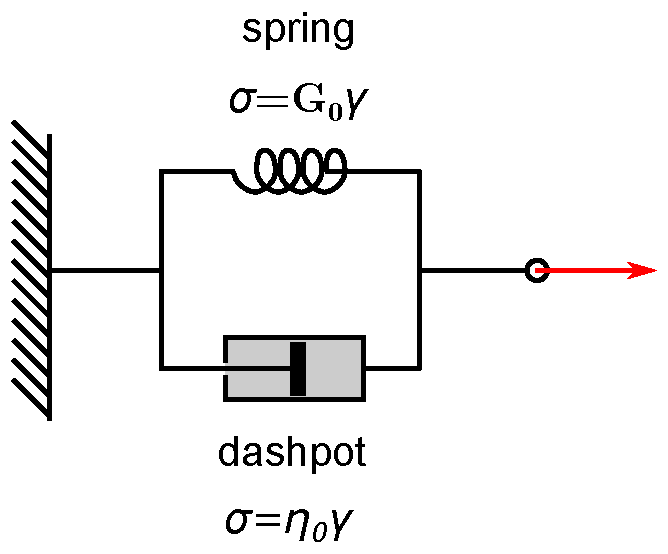
\includegraphics[width=0.4\textwidth]{\figpath/exercise-voigt}}
			
			In this case, the total \emph{stress} is the sum of the stresses across the two components, while the total \emph{strain} is identical for each component.
			
			\begin{enumerate}
				\item Express the above statement using appropriate mathematical equations. 
				
					\begin{solution}\instructordisplay{
						Total stress:
						\begin{equation*}
							\sigma_{Voigt} = \sigma_{spring} + \sigma_{dashpot}
						\end{equation*}
						
						Total strain:
						\begin{equation*}
							\epsilon_{Voigt} = \epsilon_{spring} = \epsilon_{dashpot}
						\end{equation*}
					}\end{solution}
					
				\item When considering the Voigt model, we usually consider its response to an increase in stress rather than an increase in strain.
				
					A step-stress stress profile is shown below:
		
					\vspace{3pt}
					\centerline{\hspace{2.5cm}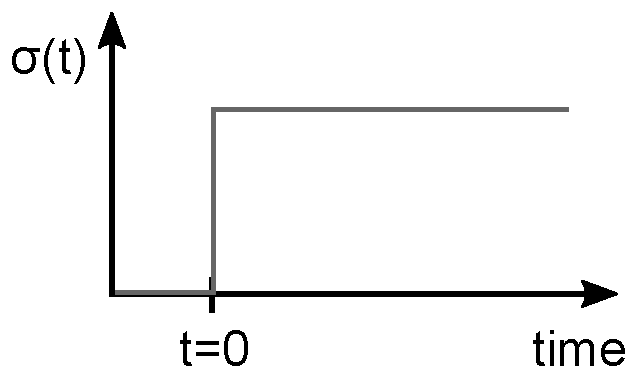
\includegraphics[width=0.35\textwidth]{\figpath/step-stress-profile}}
					
					\begin{enumerate}
						\item What do you expect to happen in the instant immediately after the stress (force) is applied?
						
							\begin{solution}\instructordisplay{
								Immediately after the force is applied, nothing will happen, because the dashpot cannot deform instantaneously.  All of the stress will be held by the dashpot, and none by the spring.
							}\end{solution}
						
						\item What do you expect to happen as you continue to apply the force?
						
							\begin{solution}\instructordisplay{
								Over time, the dashpot will begin to relax (deform), and the spring will begin to extend.  As $t\to\infty$, all of the stress will transfer to the spring, and the final strain will just be $\gamma(t\to\infty) = \sigma_0/G_0$, where $\sigma_0$ is the magnitude of the applied stress.
							}\end{solution}
						
						\item Sketch the strain that you would expect to measure as a function of time:
			
				\begin{solution}[1.5in]
					\studentdisplay{
						\vspace{6pt}
						\centerline{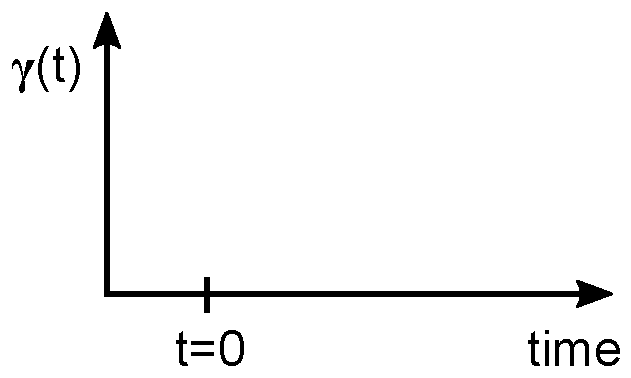
\includegraphics[width=0.4\textwidth]{\figpath/exercise-voigt-strainresponse-blank}}
						\vspace{6pt}
					}
					\instructordisplay{
						\vspace{6pt}
						\centerline{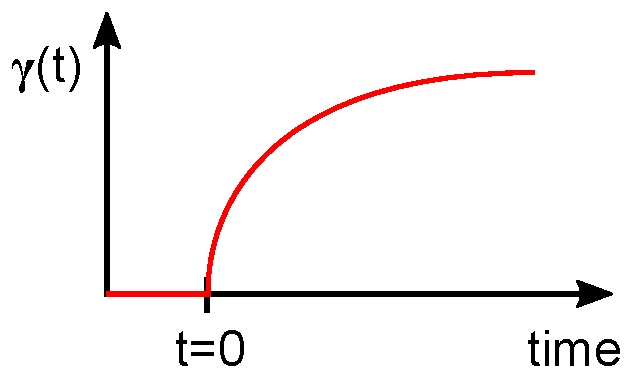
\includegraphics[width=0.4\textwidth]{\figpath/exercise-voigt-strainresponse-solution}}
						\vspace{6pt}
					}
				\end{solution}
					\end{enumerate}
			\end{enumerate}
		
\end{exercises}
	
\end{activity}